\documentclass[12pt,a4paper,twoside]{article}
\usepackage[utf8]{inputenc}
\usepackage[spanish,es-lcroman,es-nosectiondot]{babel}%quitar el punto después de secciones
\usepackage[style=english]{csquotes}
\usepackage[T1]{fontenc}

\usepackage{mathtools}

\usepackage{titlesec}
\titleformat*{\section}{\normalsize\bfseries}
\titleformat*{\subsection}{\normalsize\bfseries}
\titlespacing\section{0pt}{12pt plus 4pt minus 2pt}{0pt plus 2pt minus 2pt}%espaciado entre secciones y subsecciones
\titlespacing\subsection{0pt}{12pt plus 4pt minus 2pt}{0pt plus 2pt minus 2pt}
\titlespacing\subsubsection{0pt}{12pt plus 4pt minus 2pt}{0pt plus 2pt minus 2pt}

\usepackage[margin=1in]{geometry}
\setlength{\parindent}{0.5in}
\setlength{\parskip}{1em}
\usepackage{caption}
\usepackage{subcaption}
\captionsetup{figurename=\textit{Figura},tablename=\textit{Tabla}}
\renewcommand\thefigure{\textit{\arabic{figure}}}


\usepackage[style=authoryear,backend=biber,citestyle=apa,maxnames=2]{biblatex}
\DefineBibliographyStrings{spanish}{andothers={et~al\adddot}}%et al en vez de y cols.
\addbibresource{estadbiblio.bib}

\usepackage[title,titletoc]{appendix}%para poner apéndice
\usepackage[dotinlabels]{titletoc}%para hacer referencias

\usepackage{pdflscape}

\usepackage{amsmath,amssymb}
\usepackage{graphicx}
\usepackage{float}

\usepackage[spanish]{cleveref}
\crefname{section}{§}{§§}
\Crefname{section}{§}{§§}
\crefname{subsection}{§}{§§}
\Crefname{subsection}{§}{§§}
\crefname{subsubsection}{§}{§§}
\Crefname{subsubsection}{§}{§§}

\usepackage{perpage} 
\MakePerPage{footnote}
\usepackage{scrextend}
\deffootnote{1em}{1.6em}{\thefootnotemark\enskip}

\usepackage{pgfplots}
\pgfplotsset{axis lines=middle,
            width=\textwidth,
            height=8.5cm,
            compat=newest,
            xlabel shift={6.5em},
            ylabel shift={-1em}
            }            
            
\usepackage{fancyhdr}
    \pagestyle{fancy}
    \fancyhf{}
     \fancyhead[LO]{\slshape{\textbf{\MakeUppercase{Análisis de Rentabilidad en el Ecuador}}}}
     \fancyhead[RO]{\Large{\LaTeX}}
     \fancyhead[LE]{\textsc{Daniel Sánchez}}
     \fancyhead[RE]{\textsc{Estadística II}}
     \fancyfoot[CO,CE]{-\thepage-}
     

     
\usepackage{setspace}
\onehalfspacing

\begin{document}
\pagenumbering{roman}
    \begin{titlepage}
        \begin{center}
            \vspace*{1cm}
            \line(1,0){400}\\
            \Huge{\textsc{{\textbf{Proyecto No. 1}}}}\\
            \Huge{\textsc{Análisis de Rentabilidad en Empresas Ecuatorianas}}\\
            \line(1,0){400}\\
            \vspace*{1cm}
            \Large{Daniel Sánchez}\\
            \Large{00138542}\\
            \large{Quito, 24 de octubre de 2018}\\
        \end{center}
    \vspace*{8cm}
    Estadística II\\
    Jessica Hidalgo \\
    NRC 3833\\
    LI 10:00-11:20\\
    Semestre I 2018-2019\\
    Universidad San Francisco de Quito
    \clearpage

\end{titlepage}
\pagenumbering{roman}
\begin{abstract}

Este trabajo se propuso a realizar un análisis de la rentabilidad, o capacidad de crear valor agregado, de las empresas y establecimientos de la economía ecuatoriana. Los datos utilizados han sido aquellos del en el ejercicio fiscal del 2017, el período más reciente para el cual se tiene indicadores financieros para las empresas que mantienen una relación con el Estado o que constan en el directorio de compañías de la Superintendencia de Compañías, Valores y Seguros.  

El análisis, de carácter cuantitativo, estuvo en todo momento orientado a la formación de conclusiones que se apliquen al ámbito macroeconómico actual, que ha sido sujeto a extenso análisis debido a los últimos años recesivos para la economía y tras el cambio paradigma económico y político que existió tras el cambio de administración ejecutiva en el año 2017. 

Por esto, se tomó en cuenta dos sectores de la economía ecuatoriana, comercio y servicios, que son los más numerosos en establecimientos. A través de un muestreo aleatorio simple, se llevaron a cabo pruebas de comparación de medias y varianzas, para determinar cual de estos sectores es más rentable financieramente, y formar conclusiones más generales sobre la operación de los establecimientos y la naturaleza del sector económico.

El indicador financiero que se utilizó fue la rentabilidad financiera como se calcula para la Superintendencia de Compañías, Valores y Seguros; para poder tener en mente la rentabilidad que se genera después de haber deducido de ésta todos los impuestos y otros gastos de carácter ajeno a lo operacional. Todos estos gastos, y también ingresos, mantienen gran importancia económica en el Ecuador debido a la legislación actual en el ámbito empresarial. De esta manera, se evalúa de manera general como las empresas aportan valor agregado a la economía, considerando todas sus fuentes de ingreso y gasto. El muestreo realizado fue de quince empresas del sector Servicios y el sector Comercio, seleccionadas aleatoriamente. 

Todos los cálculos fueron realizados en Minitab 17. La sesión de trabajo fue impresa y adjuntada al final del trabajo.

Las pruebas de comparación de medias y de varianzas trajeron a la luz los hechos de que la empresa de servicios promedio es más rentable que la empresa promedio de comercio. Las implicaciones se ven respaldadas por tasas de cambio anual en el producto interno bruto y consideraciones de modelos macroeconómicos. 

\end{abstract}
\clearpage

\tableofcontents
\listoffigures
\listoftables
\clearpage

\pagenumbering{arabic}

\section{Introducción}\label{sec:intro}

La historia del país demuestra que a lo largo de los años la economía ecuatoriana se ha desenvuelto en una escala relativamente pequeña en América Latina, dependiente de la producción de materia prima para su exportación a países con capacidades de procesamiento y manufactura. Uno de los puntos críticos de la economía fue la crisis de finales de los años noventa, en donde, debido a una profunda crisis financiera y monetaria, se reemplazo a la moneda nacional conocida como el sucre por el dólar americano \parencite{dolarbce}.

No solamente se vería una gran inestabilidad económica, sino también la caída de tres gobiernos en solo nueve años. La inestabilidad política terminaría en 2007 con la elección de Alianza \textsc{Pais} \parencite{20002014inec}. La elección del nuevo Gobierno implicaría un radical cambio a la ideología política económica que se había utilizado anteriormente:
\blockquote{
    \ldots la encendida indignación popular le siguió un gran rechazo electoral a la vieja partidocracia, eligiendo a la Revolución Ciudadana como otra forma de hacer política \ldots Un hito histórico que en el plano económico supuso una ruptura decisiva con las ataduras del pensamiento único de corte neoliberal y su renovación por postulados económicos heterodoxos \ldots \parencite[pp.~11-12]{paislibro} 
    }
Sin embargo, si bien existieron algunos cambios positivos para el país en el período del gobierno socialista, el efecto de las decisiones tomadas en dicho período ha sido ampliamente debatido y estudiado, donde varios juicios de valor toman lugar. Lo cierto es que actualmente la economía sufre un período de estancamiento al haberse acostumbrado a precios competitivos del petróleo y a un gasto público desproporcionado \parencite{ladesaceleracioncorporaciondeestudiosparaeldesarrollo, elcrecimientocorporaciondeestudiosparaeldesarrollo,cuestionesbce, laeramosquera&vaca}.

\textcite{hechosluciopablo} señala que el radical cambio fue un aumento del rol del gobierno en la economía como un organismo regulador de tanto consideraciones económicas como sociales, que afectó a la economía de diversas maneras. Si bien el cambio pareció ser positivo en varias maneras, la mala administración de fondos obtenidos durante la época de bonanza petrolera causó una profunda crisis económica, a ser manejada por la administración nueva, elegida a mediados del 2017 \parencite{latrampalatorre&hidalgopallares}. El nuevo gobierno parece estar decidido al cambio de lo anterior, mediante medidas económicas de ahorro, promoviendo la política neoliberal que el anterior gobierno había desafiado abiertamente \parencite{deficitfiscaldavalos}, pero con un efecto que difícilmente puede ser calificado como positivo a largo plazo \parencite{elcrecimientocorporaciondeestudiosparaeldesarrollo}.

La crisis económica que tomó lugar después del 2014 tiene sus raíces en la bonanza que se dio desde el 2003 debido a altos precios de \textit{commodities}\footnote{Los \textit{commodities} son la materia prima utilizada para la producción de otros bienes, dependientes de fuerzas naturales, por ejemplo: el petróleo, el gas natural, carbón, etc. \parencite{commoditiesdemystifiedtrafigura}.}, hasta el fin de esta bonanza en 2013 \parencite{ladesaceleracioncorporaciondeestudiosparaeldesarrollo}. Los ciclos económicos e ingresos públicos de varios países latinoaméricanos son dependientes en la exportación de \textit{commodities}, y el efecto de una reducción del precio afecta más a los países que más dependen de estas exportaciones, y el Ecuador es uno de estos casos \parencite{cuestionesbce}. La figura \ref{fig:flujoec} muestra las variaciones porcentuales anuales del PIB\footnote{El PIB es una medida macroeconómica utilizada para medir el bienestar económico de un país. \parencite{principiosdemankiw}.} real de la economía ecuatoriana.\par
\begin{figure}[H]
\fbox{
\begin{minipage}{\textwidth}
    \pgfkeys{/pgf/number format/.cd,1000 sep={}}
    \centering
    \vspace{1em}
    \begin{tikzpicture}
    \begin{axis}[font=\small,
        xlabel={Período [Años]},
        ylabel={Crecimiento anual [\%]},
        xmin=1985, xmax=2018,
        ymin=-10, ymax=+12,
        xtick={1987,1990,1995,2000,2005,2010,2015,2017},
        ytick={-10,-8,-6,-4,-2,0,2,4,6,8,10},
        legend pos=south west,
        ymajorgrids=true,
        xmajorgrids=true,
        grid style=dashed,
        ]
    \addplot[smooth,
        color=blue,
        mark=square,
        ] coordinates{(1987,-6)(1988,10.5)(1989,0.3)(1990,3)(1991,5)(1992,3.6)(1993,2)(1994,4.7)(1995,1.75)(1996,2.4)(1997,4.05)(1998,2.12)(1999,-6.3)(2000,2.8)(2001,5.34)(2002,4.25)(2003,3.58)(2004,8)(2005,4.1)(2006,3.4)(2007,4.3)(2008,0.8)	(2009,2.9)(2010,0.7)(2011,7.5)(2012,-0.5)(2013,6.4)(2014,5.9)(2015,2.1)(2016,0.2)(2017,4.4)};
        \legend{Variación del PIB}
         \end{axis}
    \end{tikzpicture}
    \caption[Variaciones porcentuales del PIB real 1987-2017]{Variaciones anuales porcentuales del PIB real respecto al año anterior durante los últimos 30 años. Datos recuperados del boletín de Información Estadística Mensual, Banco Central del Ecuador \parencite*{iembce}. Elaborado con el paquete \LaTeX \ \textsf{pgfplots}.}
    \label{fig:flujoec}
    \end{minipage}
    }
\end{figure}
Es clara una áspera caída del PIB en 1999, para luego ver una recuperación en los siguientes años, con caídas en períodos de crisis mundial y finalmente la crisis nacional que ha sido mencionada anteriormente. La \textcite{ladesaceleracioncorporaciondeestudiosparaeldesarrollo} prevee que el crecimiento económico del 2018 será menor al del 2017, y no descarta la posibilidad de una recesión\footnote{Período en la economía donde el ingreso real disminuye, causando complicaciones en otros ámbitos económicos y sociales \parencite{principiosdemankiw}.} debido a la aún presente dependencia en el gasto público, que ha disminuido desde el cambio de administración.

Uno de los varios agentes económicos perjudicados por las recesiones del país, sea cual haya sido, es la empresa privada. Una desaceleración de la economía puede producir inflación de varias maneras, como fue el caso del Ecuador debido a una inyección monetaria a las instituciones financieras \parencite{memoriaanualbancocentraldelecuador}, y la inflación afecta a las empresas en reducciones de su ingreso real y aumentos de sus gastos.

La relación de la empresa, vista como una unidad económica independiente, puede ser poco clara en cuanto a su relación al PIB. Sin embargo, según \textcite{macroeconomicsmankiw}, el PIB mide, además de el conjunto de producción total de un país y la renta nacional, la suma de valores agregados de todas las empresas del país. El valor agregado es definido aquí como la diferencia entre los costos de productos intermedios o costos de producción y los valores de los productos finales; el valor añadido por la empresa a través de su trabajo. 

Se puede evaluar esto observando la producción de utilidades de una empresa, no en cuanto a magnitud simplemente, sino evaluando la capacidad de producción de utilidades en base a sus recursos, en otras palabras, su rentabilidad. Una economía desacelerada puede afectar a las empresas reduciendo su rentabilidad, es decir, \textit{reduciendo su posibilidad de producir valor agregado}. Sin embargo; esto es un proceso de doble retroalimentación: una economía en recesión afecta a la capacidad de las empresas de producir valor agregado, pero la economía desacelerada es causada por una baja producción de valor agregado por las empresas; establecimientos con mal uso de recursos no producen como deberían.

Con todo esto en mente, se podría decir que una manera de evaluar el efecto de decisiones microeconómicas en la situación macroeconómica y el efecto de consideraciones globales hacia el ámbito más específico de la economía puede ser la observación y análisis de la rentabilidad de las empresas. Es posible delimitar el alcance del trabajo para mayor precisión tomando en cuenta las rentabilidades de empresas que sean parte de los sectores más fuertes en el país, que son el sector de comercio y de servicios, de acuerdo a numerosos estudios realizado por el \textcite{directoriodeinstitutodeestadisticaycensos}.

Entender la estructura de estos sectores y la rentabilidad aportada por las empresas en éstos, en base a métodos objetivos de estadística descriptiva e inferencial, será la base para proporcionar una base cuantitativa para comenzar un debate mejor sustentado sobre la política macroeconómica en el país.

\clearpage
\section{Metodología}\label{sec:metodos}
A continuación se delimitará el alcance de los métodos empleados en este trabajo, en referencia a la manera en la que se ha recogido los datos muestrales y la metodología del cálculo de los indicadores escogidos para el análisis estadístico, entre otras consideraciones críticas para el entendimiento de las conclusiones surgidas del análisis cuantitativo realizado.

\subsection{Poblaciones y métodos de muestreo}\label{subsec:pob}
Como se ha dicho anteriormente, para poder extraer conclusiones con más relevancia a la realidad económica ecuatoriana el análisis estadístico debería realizarse a los sectores con mayor concentración de empresas y establecimientos. De acuerdo a lo expuesto por el \textcite{directoriodeinstitutodeestadisticaycensos} los sectores de la economía ecuatoriana con mas concentración de empresas y establecimientos (al año 2016) son los de Servicios y Comercio, con el 40,59\% y el 36,62\% de participación, respectivamente. A continuación, una descripción mas precisa de ambos sectores.\par
\subsubsection{Sector Servicios}\label{subsubsec:servicios}
\textcite{elsectorserrano} señala que los servicios son la actividad económica más heterogénea de las economías, y se diferencian del comercio de bienes debido a la naturaleza del consumo de estos: generalmente los servicios se producen durante el tiempo y son consumidos directamente después, ya que no pueden ser almacenados al ser intangibles. Las economías usualmente tienen un sector de servicios extremadamente grande e importante, además de que en la actualidad prácticamente cualquier actividad económica implica la existencia de un servicio.\par
Sin embargo, ya que se adoptó la agrupación de actividades económicas del INEC en el Directorio de Empresas y Establecimientos (DIEE) en el año 2016, las empresas muestreadas del sector de servicios pertenecen a determinadas actividades económicas, determinadas por la Clasificación Industrial Internacional Uniforme de actividades económicas propuesta por la ONU. Se excepciona las actividades económicas financieras, que se desconsideraron del análisis por su modelo de negocios diferente al de una empresa de servicios regular.

\subsubsection{Sector Comercio}\label{subsubsec:comercio}
Lo que se entiende por el sector comercio por el INEC sí se considera una actividad económica independiente por la CIIU y la define de la siguiente manera: 
\enquote{
    \ldots el comercio al por mayor y menor (venta sin transformación) de cualquier tipo de artículo, y la realización de servicios secundarios para la venta al por mayor y al por menor \ldots} \parencite{clasificaciondeinstitutonacionaldeestadisticaycensos}.
Sin embargo, dicha clasificación incluye el servicio de reparación y mantenimiento de automotrices; para efectos de exactitud en el análisis estadístico las empresas que se desempeñen solamente en esta subactividad han sido asignadas a la población Sector Servicios. El siguiente apartado explicará en detalle como manejaron las poblaciones para el proceso de muestreo.

\subsubsection{Método de muestreo}\label{subsubsec:muestreo}
La información proporcionada por el INEC en el DIEE en cuanto al número de empresas y establecimientos es limitada: solamente considera entidades formadas hasta el 2016 y aquellas que mantienen una relación con el Estado (registros), a saber: (1) Ventas en el SRI, (2) Personal afiliado en el IESS I (3) Pertenecen al RISE y pagaron impuesto sobre su renta. Pueden existir unidades económicas que se desempeñen en el ámbito completamente informal y hasta ilegal que de todas maneras contribuyen a la economía indirectamente. Todas estas consideraciones hacen entender que la población de este estudio se podría caracterizar como infinita según \textcite{estadisticaanderson}, requiriendo así un muestreo aleatorio.

Sin embargo, fue complicado realizar el proceso de muestreo directamente desde el directorio de empresas de la SUPERCIAS, debido el dificultoso manejo que dichas bases de datos requerían. Además, se corría el riesgo de tomar puntos de muestra que sean \textit{empresas fantasma}\footnote{Personas jurídicas que no representan una unidad económica contribuyente, sino entidades mas bien utilizadas para transacciones entre personas naturales o jurídicas, comúnmente para fines ilícitos \parencite{directoriodeinstitutodeestadisticaycensos}.} o empresas que constaban como activas pero se encuentran en proceso de disolución. Por ello, se ha decidido utilizar el Ranking 5000 de la Revista Ekos, que clasifica las empresas más grandes del Ecuador en base a las cantidades reportadas en sus estados financieros. Los datos que se incluyen en el RK5000 son de todas maneras tomados de las bases de datos de la SUPERCIAS, la Superintendencia de Bancos y la Superintendencia de Economía Popular y Solidaria y el SRI \parencite{manualpararevistaekos}. Sin embargo se utilizan secciones algo diferentes a las de la agrupación del INEC en el DIEE, que se han ajustado para tener concordancia con todo lo anteriormente expuesto.

La figura a continuación expone la estructura de la economía como se ve en la herramienta de la Revista Ekos:
\begin{figure}[H]
\fbox{
\begin{minipage}{\textwidth}
    \centering
    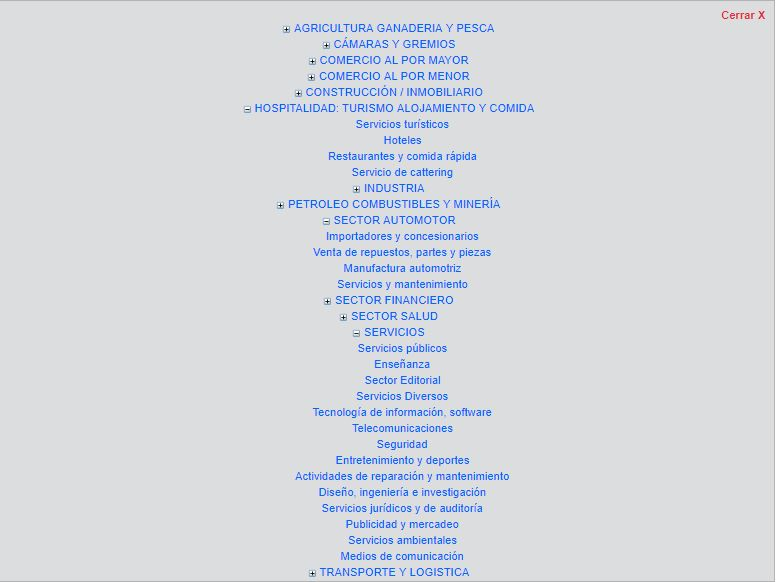
\includegraphics[scale=0.6]{ekos.JPG}
    \caption[Sectorización de la economía según la Revista Ekos (2017).]{Sectorización de la economía según la Revista Ekos en la herramienta Guía de Negocios Ranking TOP5000. Recuperado de Revista Ekos (2017).}
    \label{fig:ekos}
    \end{minipage}}
\end{figure}
Teniendo esto en consideración, las actividades económicas (como constan en el RK5000) agrupadas entre las poblaciones Sector Servicios y Sector Comercio se distribuyen de la siguiente manera:
\begin{itemize}
      \item Para el Sector Servicios, se utilizaron además los sectores  de Servicios ; Hospitalidad : Turismo, Alojamiento y Comida; Servicios y Mantenimiento del sector Automotriz y Transporte y Logística. El subsector de Manufactura automotriz fue dejado fuera del análisis puesto que estaría mejor mapeado al Sector Industria de la economía, que no esta siendo considerado en el trabajo.  
    \item Sector Comercio: Consta de Comercio al por mayor, al por menor, concesionarios y venta e importación de repuestos automotrices.
    \item Sector Servicios: Consta de todo el sector de servicios según Ekos: Sector Público, Enseñanza, Sector Editorial, Servicios Diversos, Tecnología de información, software, Telecomunicaciones, Seguridad, Entretenimiento y deportes, Actividades de reparación y mantenimiento, Diseño, ingeniería e investigación, Servicios jurídicos y de auditoría, Publicidad y mercadeo. Servicios ambientales y Medios de comunicación \parencite{manualpararevistaekos}.
  \end{itemize}

Se elaboró una lista con las empresas de RK5000 que constaban en estas secciones del ranking y se les asigno un número de orden alfabético. Se selecciono 15 números aleatorios a través de la función RAND.BETWEEN() de Microsoft Excel, y así se constituyó la muestra para cada sector en cuestión. 

\subsection{Variable analizada}

El indicador financiero de rentabilidad que se utilizará sera la rentabilidad financiera o rentabilidad sobre el patrimonio. Este indicador analiza la cantidad de retornos que cada activo financiado por los propietarios de la empresa produce. Se conoce a este indicador por \textsc{Roe}, por sus siglas en inglés, \textit{return on equity} \parencite{rentabilidad:laolivares}. Se suele conocer también como \textit{rendimiento sobre el capital} o rentabilidad sobre el patrimonio \parencite{contahorngren}, sin embargo se suele referir a este indicador como rentabilidad financiera puesto que arroja la razón en la que se produce riqueza a raíz de la inversión en recursos financieros. La fórmula general, como la propone \textcite{rentabilidad:laolivares}, se define como sigue: \par
\begin{equation}\label{equation:1}
    \text{Rentabilidad financiera}=\frac{\text{Utilidad \ del ejercicio}}{\text{Patrimonio}}
\end{equation}
Sin embargo, existen varias maneras de expresar a (\ref{equation:1}), desagregando ciertos componentes que forman la utilidad o el patrimonio, obteniendo así diferentes expresiones para el mismo indicador. La \textcite{metodologiaindicadoresfinancierossuperintendenciadecompanias} define su metodología de cálculo de la rentabilidad financiera como sigue:
\begin{equation}\label{eq:1}
    \text{Rentabilidad financiera}= \frac{\text{Ventas}}{\text{Activo}} \cdot \frac{\text{UAII}}{\text{Ventas}} \cdot \frac{\text{Activo}}{\text{Patrimonio}} \cdot \frac{\text{UAI}}{\text{UAII}}\cdot \frac{\text{Utilidad Neta}}{\text{UAI}}
\end{equation}
Donde: \textit{UAII}: utilidad antes de impuestos e intereses, \textit{UAI}: utilidad antes de impuestos y \textit{Utilidad Neta}: utilidad después del 15\% de trabajadores e impuesto a la renta. 

Para este indicador, un valor de 1 indica que por cada dólar invertido en activos para la empresa aporta 1 dólar en utilidades netas. Es posible obtener valores negativos en este indicador debido a posibles pérdidas de un ejercicio, o como la SUPERCIAS (s.f.) advierte: \blockquote{\ldots este indicador puede ser negativo debido a que para obtener las utilidades netas, las utilidades del ejercicio se ven afectadas por la conciliación tributaria, en la cuál, si existe un monto muy alto de gastos no deducibles, el impuesto a la renta tendrá un valor elevado, el mismo que, al sumarse con la participación de trabajadores puede ser incluso superior a la utilidad del ejercicio (p. 12).} 

Se ha escogido este indicador puesto que retrata fielmente la realidad del negocio; si bien se podría haber seleccionado un indicador como la rentabilidad operacional del patrimonio para poder evaluar la toma de decisiones de los administradores, existen varios agentes económicos que dependen en el ingreso financiero (así como otros que se ven severamente afectados por el gasto financiero) por tanto sería inadecuado dejar una tan importante variable fuera del análisis. Para delimitar el alcance del proyecto no se utilizó la rentabilidad sobre el activo, que incluye la generación de utilidades netas de la deuda (pasivos).
\clearpage
\section{Datos}
Los resultados del proceso de muestreo se ven retratados en la siguiente tabla:
\begin{table}[H]
\begin{center}
\begin{tabular}{|c|c|c|} \hline 
  \textbf{Denominación} & \textbf{Sector} & \textbf{RF} \\ \hline
 METALKING & Servicios & 0,36 \\ 
  MOORE STEPHENS \& ASOCIADOS & Servicios & 0,22 \\ 
  ECLIPSOFT & Servicios &  0,52 \\ 
  CENTURIOSA & Servicios & 0,07 \\ 
  TURISMO AMORA & Servicios & 0,08 \\ 
  EBF CARGO & Servicios & 0,09 \\ 
  TRANSOCEANICA & Servicios & 0,68 \\ 
  TRANSVELEZORTIZ & Servicios & 0,19 \\ 
  ROCALVI & Servicios & 0,58 \\ 
  LAARCOM & Servicios & 0,72 \\ 
  OFFICESOLUCIONES & Servicios & 0,15 \\ 
  WORKFORCE & Servicios & 0,36 \\ 
  CENTRALIMENTOS & Servicios & 0,53 \\ 
  VASERUM CIA. & Servicios & 0,17 \\ 
  TUTTO FREDDO & Servicios & 0,26 \\
  GAMAPARTES & Comercio & 0,19 \\ 
  ESEMEC & Comercio & 0,14 \\ 
  FERREMUNDO & Comercio & 0,18 \\  
  COMPUFACIL & Comercio & 0,11 \\  
  NIKAMAR & Comercio & 0,42 \\ 
  ACERO COMERCIAL ECUATORIANO & Comercio & -0,21 \\    
  OPTICA LOS ANDES & Comercio & 0,08 \\ 
  DISTRIBUIDORA CAAMAÑO-CORNEJO & Comercio & -0,11 \\  
  PROVEMARCAS & Comercio & 0,07 \\ 
  VINESA & Comercio & 0,69 \\ 
  TRANSMARINER & Comercio & 0,56 \\  
  INSPA & Comercio &  0,23 \\ 
  TIANSHI ECUADOR & Comercio &  0,06 \\ 
  HORTICOORP ANDINA & Comercio & 0,11 \\
  TERMALIMEX & Comercio & 0,47 \\ 
    \hline
  \end{tabular} 
  \end{center}
\label{tab:tablarent}
\caption[Rentabilidades financieras de empresas muestreadas]{Rentabilidades financieras de cada una de las empresas que fueron seleccionadas por el muestreo aleatorio. Datos recuperados de \cite{indicadoresupercias} y \cite{guiaderevistaekos}, redondeados a la centésima. Nota: Se ha omitido las terminaciones (CIA LTDA., S.A.) de la tabla.}
\end{table}
A continuación, un mirada a los estadísticos descriptivos de cada muestra.
\subsection{Estadísticos: Sector Servicios}
La tabla a continuación describe los estadísticos descriptivos, calculados en Minitab 17 para esta población. \par
\begin{figure}[H]
\fbox{
\begin{minipage}{\textwidth}
    \centering
    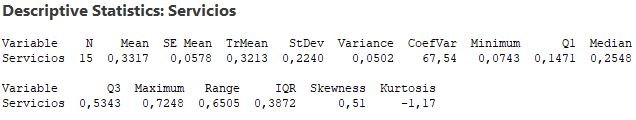
\includegraphics[scale=0.8]{statservicios.JPG}
   \caption[Estadísticos descriptivos para la población Sector Servicios]{Estadísticos descriptivos para la población Sector Servicios. Cálculos realizados en Minitab 17.}
    \label{fig:statservicios}
    \end{minipage}}
\end{figure}
El promedio de 0,33 expresa que cerca del 33\% del valor del patrimonio de estas empresas se transforma en utilidades netas, una cantidad mayor a la media muestral de la población Sector Comercio. La variabilidad parece ser menor en esta muestra: si bien la varianza es solo 0,01 menos que la varianza de comercio, el coeficiente de variación es mucho menor que el del Sector Comercio. No existen datos en la muestra con signos negativos, y el máximo de esta muestra representa la rentabilidad más alta de todas las empresas que han sido muestreadas: corresponde a la empresa LAARCOM, empresa de vigilancia y seguridad en Quito. El RIC es ligeramente mayor en esta población, el sesgo tiene exactamente el mismo valor pero la curtosis muestra que los datos están muy concentrados en la media. \par
\begin{figure}[H]
\fbox{
\begin{minipage}{\textwidth}
    \centering
    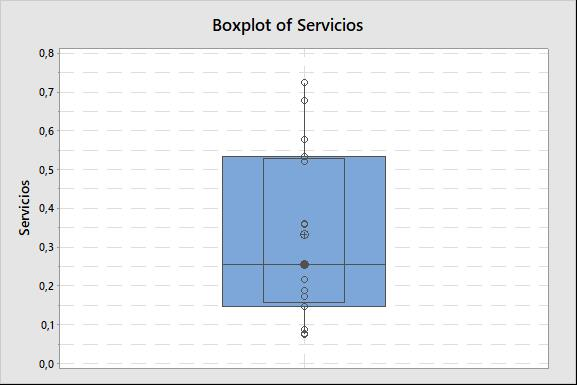
\includegraphics[scale=0.6]{boxplotservicios.jpg}
    \caption[Diagrama de caja de población Sector Servicios]{Diagrama de caja de población Sector Servicios. Elaborado con Minitab 17.}
    \label{fig:cajaservicios}
    \end{minipage}}
\end{figure}
El diagrama de caja una vez muestra la desigualdad entre media y mediana, y así mismo se observa mayor dispersión entre el 50 al 75 \% que del 25 al 50 \%.

La prueba de normalidad, planteada de la misma manera que en el Sector Comercio, dio los siguientes resultados:
\begin{figure}[H]
\fbox{
\begin{minipage}{\textwidth}
        \centering
    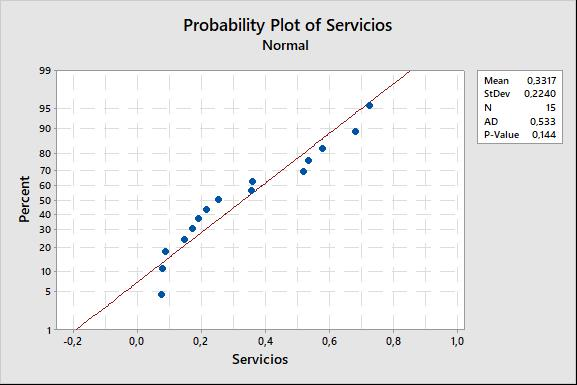
\includegraphics[scale=0.6]{normservicios.jpg}
    \caption[Prueba de normalidad de Sector Servicios]{Prueba de normalidad de Sector Servicios Elaborado con Minitab 17.}
    \label{fig:normserv}
    \end{minipage}}
\end{figure}
Al ser mayor el valor-p que $\alpha= 0,1$, no es posible rechazar la hipótesis nula de normalidad. Se puede decir que el 95\% de los datos de la población Sector Servicios se encuentran a dos desviaciones estándar de la media (entre 0,11 y 0,55 de rentabilidad financiera). Al tener en general una menor variabilidad que la otra población se puede decir que las empresas seleccionadas para el Sector Servicios son más rentables que aquellas seleccionadas para el Sector Comercio. 

Los intervalos de confianza para la media poblacional son los siguientes:
\begin{itemize}
    \item (0,2298; 0,4336) para $\alpha=0,1$
    \item (0,2077; 0,4558) para $\alpha=0,05$
    \item (0,1595; 0,5039) para $\alpha=0,01$
\end{itemize}
\subsection{Estadísticos: Sector Comercio}
La tabla a continuación describe los estadísticos descriptivos, calculados en Minitab 17.
\begin{figure}[H]
\fbox{
\begin{minipage}{\textwidth}
    \centering
    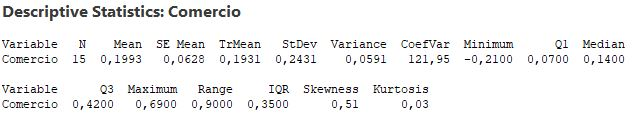
\includegraphics[scale=0.8]{statcomercio.JPG}
    \caption[Estadísticos descriptivos para la población Sector Comercio]{Estadísticos descriptivos para la población Sector Comercio. Cálculos realizados en Minitab 17.}
    \label{fig:statcomercio}
    \end{minipage}}
\end{figure}
El promedio para el sector de comercio es de 0,2 o 20\% de utilidad generada por el patrimonio de la empresa, sin embargo los datos muestran una alta variabilidad: la desviación estándar es de 0,24 representa el 122\% de la media. El RIC confirma esta aseveración afirmado que existe un 25\% de datos que toman valores por arriba de 0,42, poco menos del doble del promedio. Los valores atípicos  se hallan en la empresa ACERO COMERCIAL ECUATORIANO,  con una rentabilidad negativa del 21\%, y en la empresa VINESA, con una rentabilidad del 69\%.  El 50\% de datos se encuentra en la mitad de la distribución, con variaciones de 35 puntos porcentuales dentro de este, una vez más un número grande comparado al promedio muestral. Se ve un sesgo ligero a la derecha, y la curtosis expresa que los datos se encuentran cercanos a la media y se aproximan a una distribución normal, cuya curtosis es 0. 
\begin{figure}[H]
\fbox{
\begin{minipage}{\textwidth}
    \centering
    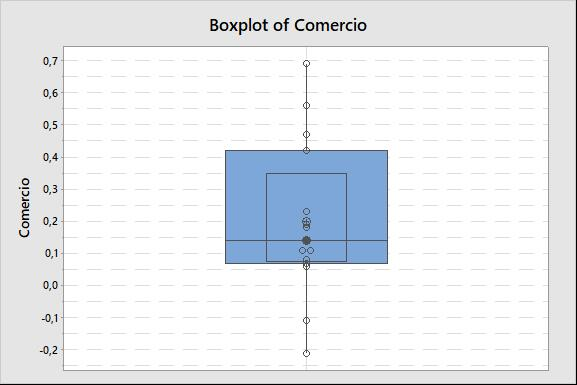
\includegraphics[scale=0.5]{boxplotcomercio.jpg}
    \caption[Diagrama de caja de población Sector Comercio]{Diagrama de caja de población Sector Comercio. Elaborado con Minitab 17.}
    \label{fig:cajacomercio}
    \end{minipage}}
\end{figure}
La figura \ref{fig:cajacomercio} confirma la variabilidad de los datos, y muestra que el promedio no es exactamente simétrico o igual a la mediana. Además, las rentabilidades que corresponden al 50 y 75 \% de la población están mucho más dispersas que el intervalo de 25 a 50 \%.

Posteriormente, se realizó una prueba de hipótesis para evaluar la normalidad de la muestra, como sigue:
$$H_{o}: \text{la población es normal}$$
$$H_{a}: \text{la población no es normal}$$
\begin{figure}[H]
\fbox{
\begin{minipage}{\textwidth}
    \centering
    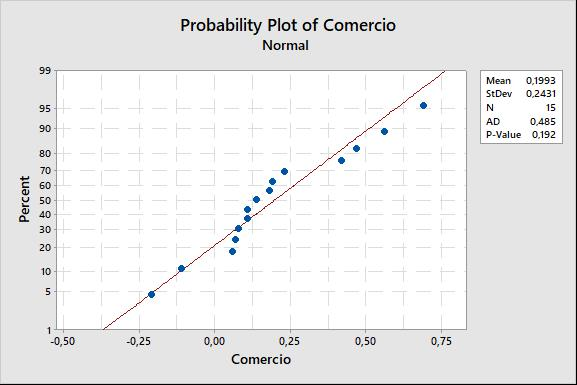
\includegraphics[scale=0.6]{normcomercio.jpg}
    \caption[Prueba de normalidad Sector Comercio]{Prueba de normalidad de la población Sector Comercio. Elaborado con Minitab 17.}
    \label{fig:normalidadcomercio}
    \end{minipage}}
\end{figure}
Dado que el valor-p es mayor a un $\alpha=0,1$, no existe suficiente evidencia estadística para afirmar que la población no esta distribuida normalmente. Por tanto, es posible inferir que un 95\% de los datos en la población se encuentran entre dos desviaciones estándar, que implica una variación de más del 200\% del valor del promedio muestral. Es posible también calcular los siguientes intervalos de confianza para la media poblacional:
\begin{itemize}
    \item (0,0888; 0,3099) para $\alpha=0,1$
    \item (0,0647; 0,3340) para $\alpha=0,05$
    \item (0,0125; 0,3862) para $\alpha=0,01$
\end{itemize}
\section{Resultados del Análisis}
\subsection{Prueba de Medias}
Para poder llegar a conclusiones globales sobre las poblaciones de comercio y servicios, fue necesario formar una prueba de hipótesis que compare ambas medias y pueda brindar conclusiones sobre la validez de las hipótesis. Puesto que, según la investigación de \textcite{directoriodeinstitutodeestadisticaycensosb}, los resultados tabulados señalan una mayor concentración de empresas y establecimientos en el sector de servicios de la economía, se entiende que debe existir un cierto tipo de atractivo a futuros emprendedores para operar en el sector de servicios antes que en otro. Este atractivo no necesariamente se traduce en una mayor rentabilidad sectorial, bien podría tratarse de un atractivo por facilidad, por amplias opciones y gran oferta laboral, sin embargo, se establecerá que la media de rentabilidad financiera es mayor en Servicios que en Comercio, y se investigará la posibilidad de lo contrario en la hipótesis alternativa. 

Por ende, se establecen las expresiones siguientes:
$$H_{o}:\mu_{1}-\mu_{2}\leq 0$$
$$H_{a}:\mu_{1}-\mu_{2}>0$$
, o bien:
$$H_{o}:\mu_{1}\leq \mu_{2}$$
$$H_{a}:\mu_{1}>\mu_{2}$$
donde $\mu_{1}$ representa a la  media poblacional de rentabilidad financiera del Sector Comercio y $\mu_{2}$ representa la media poblacional de rentabilidad financiera del Sector Servicios. Se ha definido así la prueba para poder investigar si es que el Sector Comercio en el Ecuador, más pequeño y con mas protección en el mercado (no existen cadenas extranjeras de importancia que compitan con los grandes comerciantes al por menor del país) podría ser mas rentable que el sector de Servicios.

A continuación, los resultados de la La prueba de hipótesis de dos medias con desviación estándar poblacional realizada.
\begin{figure}[H]
    \fbox{
\begin{minipage}{\textwidth}
  \centering
   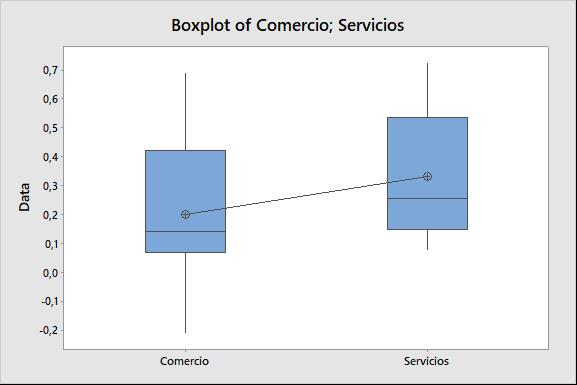
\includegraphics[scale=0.8]{boxplotambosdos.jpg}
    \caption[Diagrama de caja; Comercio vs. Servicios]{Diagrama de caja; Comercio vs. Servicios. Elaborado en Minitab 17.}
    \end{minipage}
    }
\end{figure}

\begin{itemize}
    \item Estimador puntual para la diferencia entre las medias: -0,1324; valor-p es 0,066
\end{itemize}

Los respectivos intervalos de confianza para diferentes niveles de significancia arrojados fueron los siguientes: 
 
\begin{itemize}
    \item (-0,2778; 0,0130) para $\alpha=0,1$,
    \item (-0,3075; 0,0427) para $\alpha=0,05$, 
    \item (-0,3689; 0,1041) para $\alpha=0,01$,  
\end{itemize}

La rentabilidad del sector servicios se superpone significativamente a la del sector comercio, lo suficiente para  tener la posibilidad de declarar que no existe suficiente evidencia estadística para afirmar que el Sector Comercio tiene una media de rentabilidad financiera mayor a la media del Sector Servicios, para niveles de confianza más exactos (95\% y 99\%). Para el $\alpha$ de 0,1, se puede rechazar la hipótesis nula y afirmar que el sector Comercio es más rentable que el de Servicios. 

Como es de esperarse, los intervalos de confianza se hacen más grandes a diferentes niveles de sensibilidad del análisis. Es posible concluir que el Sector de Servicios es mas rentable que el Sector de Comercio en la economía formal ecuatoriana en el año 2017. 
\subsection{Prueba de Varianzas}
Los intervalos de confianza para las varianzas poblacionales de cada población se listan a continuación, según el método de $\chi^{2}$.\par
\textbf{Comercio}:
\begin{itemize}
    \item (0,0349; 0,1259) para $\alpha=0,1$,
    \item (0,0317; 0,1470) para $\alpha=0,05$, 
    \item (0,0264; 0,2030) para $\alpha=0,01$,  
\end{itemize}
\textbf{Servicios}:
\begin{itemize}
    \item (0,0297; 0,1069) para $\alpha=0,1$,
    \item (0,0269; 0,1248) para $\alpha=0,05$, 
    \item (0,0224; 0,1724) para $\alpha=0,01$,  
\end{itemize}

Se establece una prueba de dos colas para establecer diferencias en la variabilidad de las poblaciones, de la siguiente manera: 
$$H_{o}:\sigma_{1}=\sigma_{2}$$
$$H_{a}:\sigma_{1}\neq\sigma_{2}$$
, donde $\sigma_{1}$ es la varianza del sector Comercio, que es ligeramente más grande que la del Sector Servicios. 

Las siguientes figuras despliegan los resultados calculados:

\begin{figure}[H]
\fbox{
\begin{minipage}{\textwidth}
    \begin{subfigure}[b]{0.5\textwidth}
    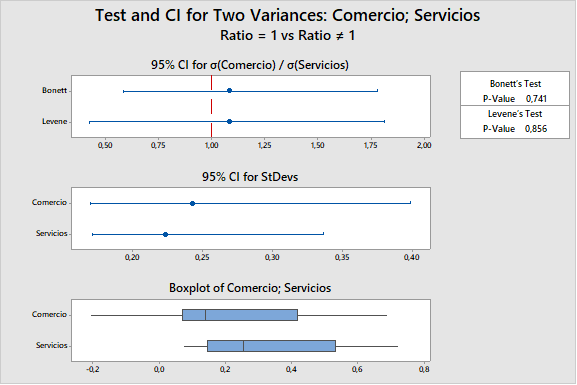
\includegraphics[width=\textwidth]{95.png}
    \caption{Prueba de varianzas de $\alpha=0,05$}
    \label{fig:f1}
  \end{subfigure}
  \hfill
  \begin{subfigure}[b]{0.5\textwidth}
    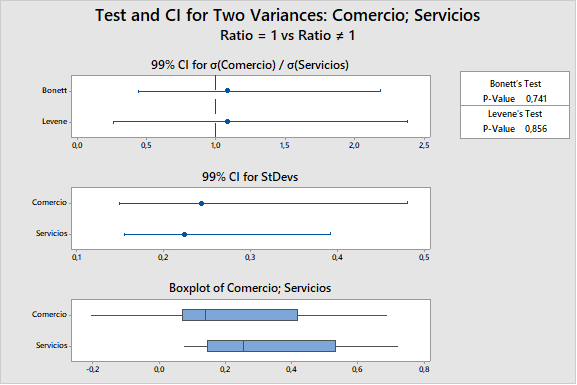
\includegraphics[width=\textwidth]{99.png}
    \caption{Prueba de varianzas de $\alpha=0,01$}
    \label{fig:f2}
  \end{subfigure}
  \caption{Pruebas de varianzas de $\alpha=0,05;0,01$; Comercio y Servicios}
  \end{minipage}}
\end{figure}
\begin{figure}[H]
    \fbox{
\begin{minipage}{\textwidth}
  \centering
   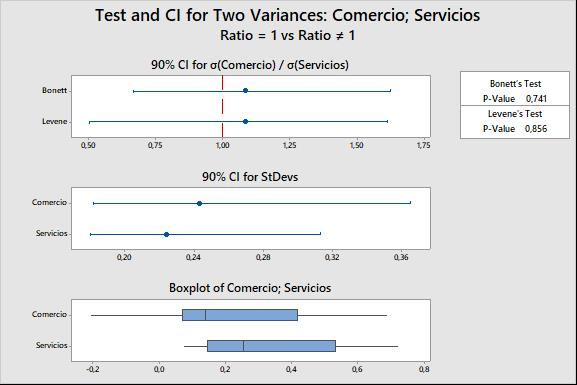
\includegraphics[scale=0.6]{90.jpg}
    \caption[Diagrama de caja; Comercio vs. Servicios]{Diagrama de caja; Comercio vs. Servicios. Elaborado en Minitab 17.}
    \end{minipage}
    }
\end{figure}

Los valores-p proporcionados por ambos métodos no son lo suficientemente pequeños como para alegar que existe suficiente evidencia estadística para aceptar la hipótesis alternativa; no se puede rechazar que las varianzas son iguales. La variabilidad entre empresas de ambas poblaciones en cuanto a su rentabilidad financiera, puesto que sus razones entre varianzas se aproximan al 1. 
\section{Discusión y conclusiones}
El hecho que se haya comprobado que el Sector de Servicios en el Ecuador es mas rentable tiene varias implicaciones: podría sugerir la existencia de una economía de escala en el sector de servicios ecuatoriano\footnote{Tipo de proceso de producción donde se aumenta los factores de producción, la cantidad producida aumenta en una proporción mayor al aumento porcentual de los factores \parencite{principiosdemankiw}}, puesto que al ser el sector de la economía con mas concentración de empresas, es claro que existe un añadido de factores de producción. El aumento de producción, con un menor gasto, causaría un mayor nivel de rentabilidad en las empresas.

Por otro lado, también puede sugerir la incidencia de otro modelo económico que se centra en la producción de un país: usualmente un país produce con eficiencia productos que requieren intensivamente de factores de producción que son abundantes en dicho país \parencite{internationaltradekrugman&obstfeld&melitz}. Con los hallazgos encontrados, esto podría realmente tener sentido, puesto que se entiende que en el Ecuador abunda el factor de producción de la labor barata o mano de obra con poca habilidad. Es posible que el tipo de servicios que se presten en este país sean servicios que mayormente no requieran de mucha experiencia, como por ejemplo puestos de trabajo de bajo nivel en empresas de transporte o de turismo. El comercio, por otra parte, si bien también requiere intensivamente de labor de poca habilidad, también requiere de capital de alta tecnología o de alto costo (para establecer redes entre proveedores y construcción de supermercados). 

Las variables macroeconómicas parecen estar a favor de la conclusión de este trabajo en cierta manera, puesto que la mayoría de industrias que pertenecen al sector de servicios han tenido tasas crecientes en el último período respecto a su participación en el producto interno bruto. 

Existieron limitaciones al proyecto aquí realizado: como se dijo, no se pudo contar con la base de datos de la propia SUPERCIAS al ser difícil de manejar (hubiera sido necesario unir más de 900.000 mil filas por archivo de Microsoft Excel, con 7 archivos, para poder crear una base de datos completa de todos los establecimientos de servicios.) y al poseer demasiados potenciales problemas, como encontrar empresas sin indicadores (estos estaban en blanco y era necesario volver a realizar un muestreo para encontrar empresas con indicadores) o encontrar empresas fantasma o en disolución. Además, no se pudo realizar un análisis estadístico más minucioso, que hubiera incluido varios procesos de muestra de la misma población y elaborar así una distribución de muestreo. Otro factor limitante fue, justamente, el actual período de ``recuperación'' de la economía: talvez encontrando un período con menos sesgos estadísticos se hubieran podido encontrar diferentes resultados. 

Para poder evaluar de manera más integral la economía se debería tomar en cuenta más sectores de los que aquí han sido evaluados; especialmente el sector de agricultura y el petrolero, que son históricamente conocidos por contribuir en la mayor proporción a la renta nacional. También se podrían evaluar otros indicadores financieros, como son los indicadores de solvencia y endeudamiento para un mejor entendimiento de la sectorización de la economía, y más indicadores o cifras de las empresa que se relacionen con el ámbito de la economía. Además, hacer una prueba estadística de las variaciones del PIB hubiera sido útil para poder compararlos con los resultados de la utilidad financiera. 

Es importante conocer como las empresas contribuyen al proceso económico nacional; el país ha recibido duros golpes en las últimas décadas, no solo económicos sino también sociales, y una de las maneras de mejorar el bienestar general de un país es mejorando su bienestar económico.
\clearpage

\printbibliography
\end{document}
